\section{Introduction}
\label{sec:introduction}

Recent years have experienced explosive growth of smartphone sales and
smartphones become pervasive. By March 2013, Google has activated more than 750M
Android-based devices \cite{Google-ARM}.  Smartphones are no longer basic
devices for making phone calls and receiving text messages, but powerful
platforms with comparable functionalities to commodity PCs.  Mobile applications
provide users the functionality to access the data maintained by remote services
such as Dropbox, Facebook, and online banking. The credential-based
authentication requires the users to provide the password (PIN), which can be
figured out by the attacker via social engineering attack. The longer the length of
password, the more time consumed by the user to manually input the password.
Recently, Shukla \etal \cite{Hand-Secret} introduce a side-channel attack on
the PIN entry process on a smartphone. The attack is entirely based on the
spatio-temporal dynamics of the hands during typing to decode the typed text. It
is demonstrated that the attack breaks an average of over 85\% of the PINs in
ten attempts on a dataset of 200 videos of the PIN entry process.

Compared to the credential-based authentication, biometric authentication is
widely considered more secure. Unlike credential-based authentication
which depends on "the knowledge of user", biometric authentication relies on "the
identity of user" which is very difficult for attackers to forge.

Facial authentication is one of the popular biometric authentication techniques.
 As shown in Figure \ref{fig:dataflow}, the data flow of
facial authentication consists of three phases. First, the photo is captured by
hardware camera on smartphone.  Second, the smartphone application obtains
the photo via the OS.  Finally, the smartphone application (processes the photo
and) sends the photo (or its extracted features) to the remote server. To achieve a trusted facial
authentication, all of three phases, which are vulnerable to attacks,  should be
secured. Even if the device has a front camera, it is rarely used in practice because of
its own limitations.

\begin{figure}[htb]
	\centering
	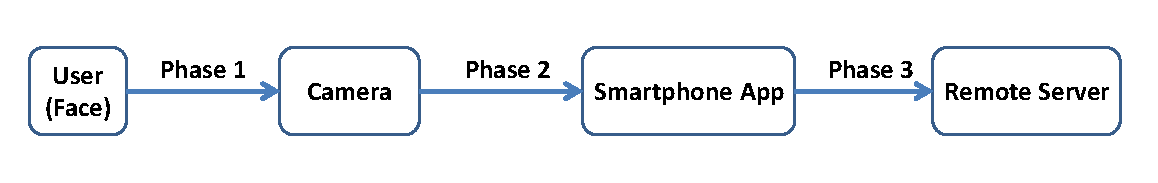
\includegraphics[width=1.0\columnwidth]{figures/dataflow.eps}
	\caption{Facial Authentication Data Flow}
	\label{fig:dataflow}
\end{figure}

\noindent
{\bf Phase 1~}
The first phase is vulnerable to 2D media attack. Instead of the real 3D face,
the attacker can easily fool the 2D face recognition by a flat photo of the
user, which is not difficult to download from social networks
\cite{android-attack}.  Although more
sophisticated 3D facial authentication techniques have been proposed to achieve
higher security \cite{Chaua-3D, Blanz-3D},  the image processing always consumes
a lot of time and the ease of use is also compromised.  For instance, to
differentiate a real 3D face from a flat photo, the Toshiba Face Recognition
Utility requires users to turn their heads towards four directions according to
a sequence of arrows shown on the screen, and the whole authentication process
takes about 30 seconds.  In this paper, we leverage the solution
proposed by Chen \etal in \cite{Chen-Sensor} to secure the first phase. Besides
the user photo, accelerometer is employed to infer the position and orientation
of the front camera. A small movement of the cellphone is applied to ensure a
real 3D face. Although the proposal of \cite{Chen-Sensor} is more efficient than 3D
facial authentication, it is still vulnerable in the second phase. 

\noindent
{\bf Phase 2~}
In the second phase, the photo (video) is retrieved by the smartphone application via
the legacy OS. On the smartphone, the large TCB of legacy OS, e.g., Android,
makes it vulnerable to malwares.  The untrusted legacy OS would tamper the
photo/video captured by the camera (e.g., virtual camera attack), or replace the
captured photo/video with pre-captured ones. Although Chen \etal
\cite{Chen-Sensor} propose Motion Vector Correlation, that is, to extract the
non-intentional shakes of user from both the video and accelerometer, and to
verify if they are correlated with each other, they assume the legacy OS is
trusted, that is, the attacker is not able to tamper the collected data at OS
level.  Besides, the computation overhead of Motion Vector Correlation is also
relatively high. To overcome the limitation in \cite{Chen-Sensor}, we leverage the
ARM TrustZone technology to ensure the trust of data from camera/accelerometer.
Both photo and accelerations are collected in TrustZone secure world.  Attackers
even with root privilege in legacy OS would not be able to compromise the
integrity and freshness of the collected data. The performance overhead of
TrustZone world switch is trivial compared to Motion Vector Correlation in
\cite{Chen-Sensor}.

\noindent
{\bf ARM TrustZone~}
TrustZone is a security extension introduced by ARM. The basic idea is to
logically partition the computing platform into two execution domains: the
normal world and the secure world.  To facilitate context switch between the two
worlds, monitor mode is introduced as the only entry point from normal world to
secure world.  Execution in the normal world jumps to the secure world by
explicitly issuing the Secure Monitor Call (SMC) instruction.  The secure world
can access the full range of the physical memory and all hardware peripherals.
On the other hand, some physical memory ranges and hardware peripherals can be
restricted to be only accessed by the secure world. Therefore, these secure
physical memory and hardware peripherals are under full hardware-based
protections from attacks that can potentially compromise the normal world legacy
OS.  Besides, interrupts and DMA are also world-aware.

\noindent
{\bf Phase 3~}
In the third phase, the photo (or features extracted from photos) is sent to the remote service to
authenticate the user. As this phase can be secured by SSL/TLS, we will not
discuss the detail in the paper.

In this paper, we propose TrustFA, a TrustZone-assisted facial authentication
to secure all three phases mentioned above.  The capture of photo, the
collection of accelerations, and the encryption/decryption of related data are
performed in TrustZone secure world.  As all of the secure world memory,
peripherals and interrupts are isolated from normal world legacy OS, attackers
even with root privilege in legacy OS would not be able to break the
authentication.  In summary, we make the following contributions in the paper: 
\begin{itemize}
\item We propose TrustFA, a TrustZone-assisted facial authentication.  Within
our knowledge, this is the first effort that all three phases in facial
authentication are secured. Compared to prior works, especially
\cite{Chen-Sensor}, the threat model regarding smartphone facial authentication
assumed in this paper is the most strongest.

\item As we leverage ARM TrustZone to ensure the trust and freshness of
camera/accelerometer data source, the performance overhead of securing Phase 2 is
only the overhead of TrustZone switch.  The future work only needs to
focus on how to more efficiently prevent 2D media attack.

\item Since the prototyping is still in progress, we envision the implementation of TrustFA on Freescale i.MX53 Quick Start
Board (QSB). We demonstrate the preliminary performance evaluation of TrustZone
world switch. Our vision is also applicable on other ARM development boards.
\end{itemize}
